The following is a simple demo case of the application, where the goal is to build a lego figure, called ``Space Pirate'', seen in Figure~\ref{}. The components ill already be partially assembled in order to reduce the number of slides a bit, as the general idea of the application will still be presented. There are four different components used to construct the Space Pirate, which can be seen in Figure~\ref{demoCaseRaw}.

	\begin{figure}[ht!]
		\centering
		\subfloat[Steering.]{{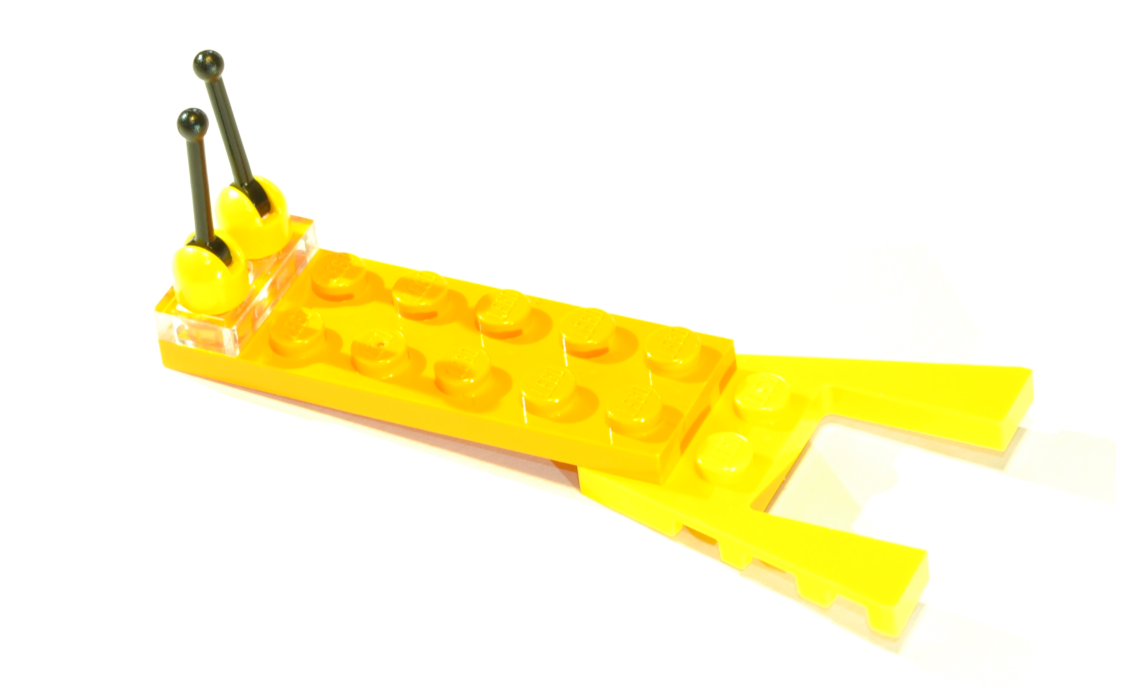
\includegraphics[width=70mm]{images/rawImages/BILD_1}}}
		\qquad
		\subfloat[Tail Light.]{{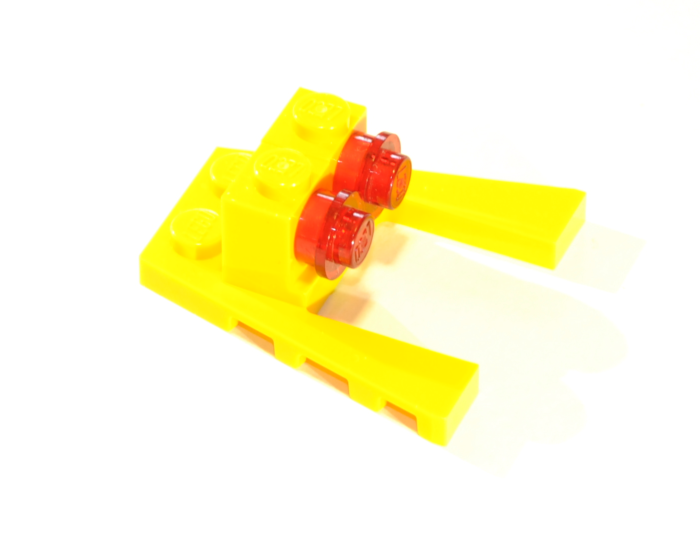
\includegraphics[width=70mm]{images/rawImages/BILD_2}}}
		\qquad
		\subfloat[Body.]{{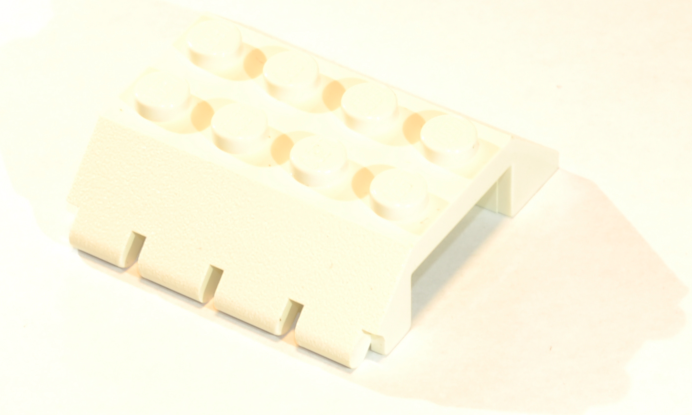
\includegraphics[width=70mm]{images/rawImages/BILD_3}}}
		\qquad
    		\subfloat[Pirate.]{{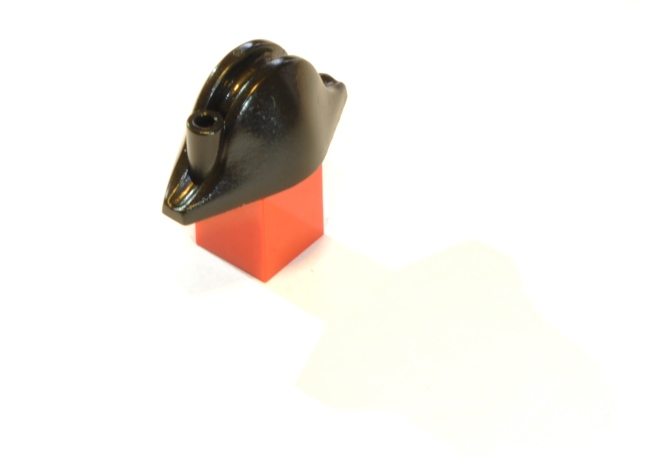
\includegraphics[width=70mm]{images/rawImages/BILD_4}}}
		\qquad
		\caption{todo.}
		\label{demoCaseRaw}
	\end{figure}

In order to receive any information on the product the user must scan the product specific QR code as seen in Figure~\ref{}. When the QR code has been scanned the information will be downloaded from the server, as seen in Figure~\ref{}. 

The first slide the user sees, when the product information has been downloaded and is being displayed to the user, is the title slide. The title slide for the Space Pirate can be seen Figure~\ref{} and shows the name of the product, as well as an image of what the product will look like when constructed.





	\begin{figure}[ht!]
		\centering
		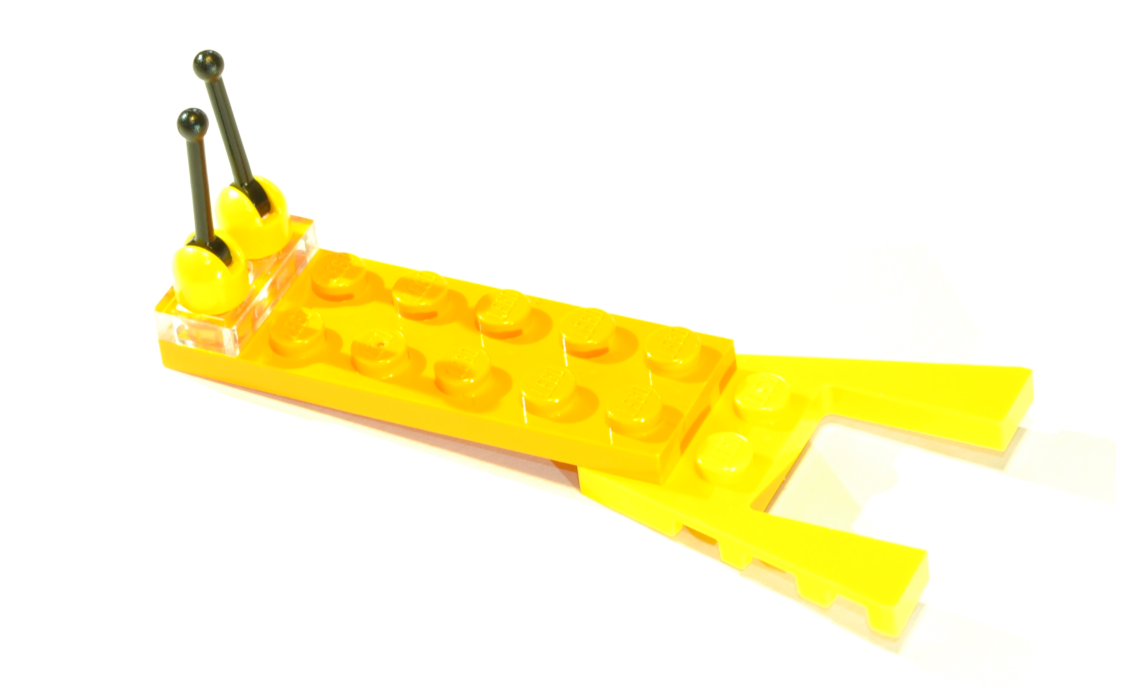
\includegraphics[width=90mm]{images/rawImages/BILD_1}
		\caption{todo.}
		\label{todo}
	\end{figure}
	
	\begin{figure}[ht!]
		\centering
		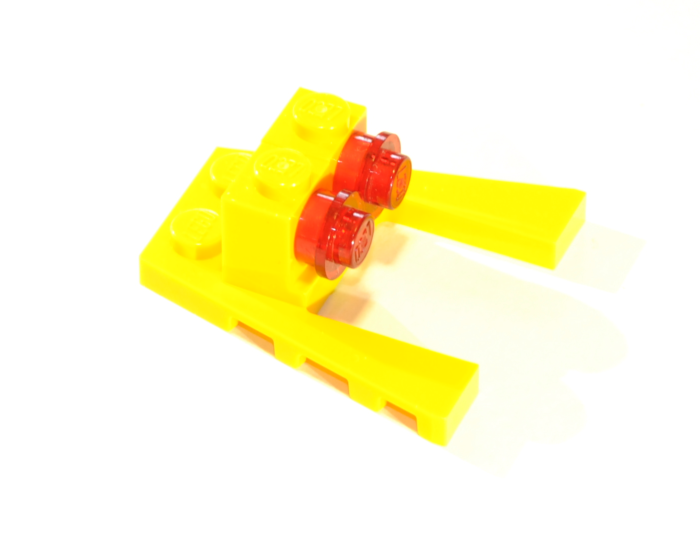
\includegraphics[width=90mm]{images/rawImages/BILD_2}
		\caption{todo.}
		\label{todo}
	\end{figure}
	
	\begin{figure}[ht!]
		\centering
		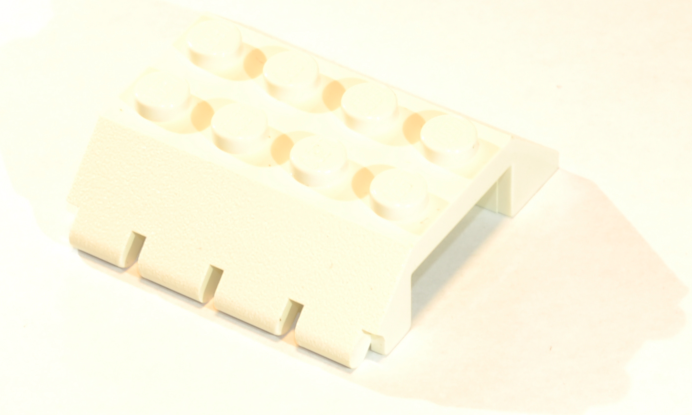
\includegraphics[width=90mm]{images/rawImages/BILD_3}
		\caption{todo.}
		\label{todo}
	\end{figure}
	
	\begin{figure}[ht!]
		\centering
		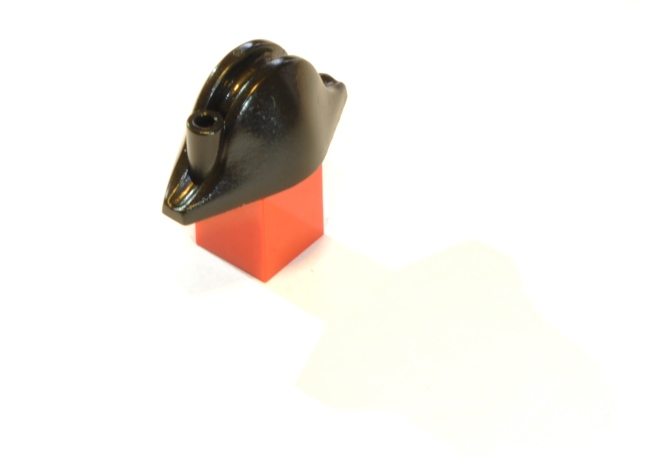
\includegraphics[width=90mm]{images/rawImages/BILD_4}
		\caption{todo.}
		\label{todo}
	\end{figure}
	
	\begin{figure}[ht!]
		\centering
		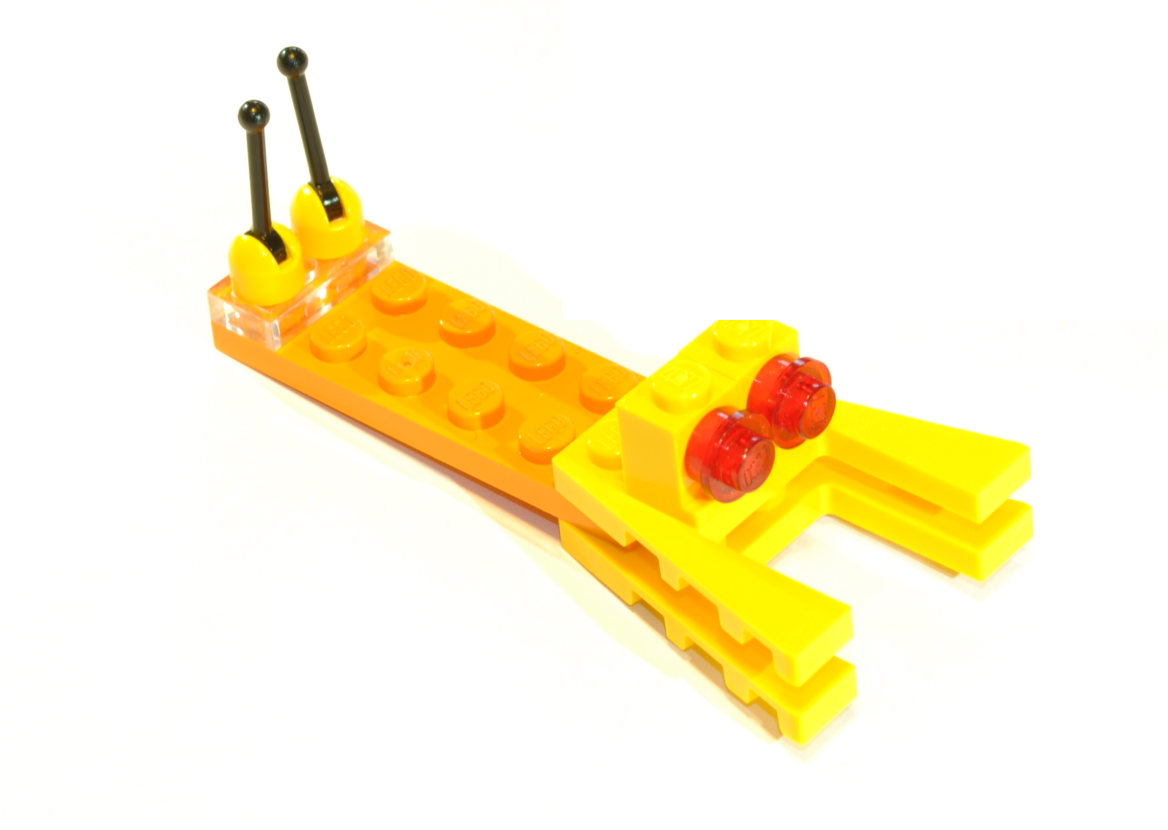
\includegraphics[width=90mm]{images/rawImages/BILD_5}
		\caption{todo.}
		\label{todo}
	\end{figure}
	
	\begin{figure}[ht!]
		\centering
		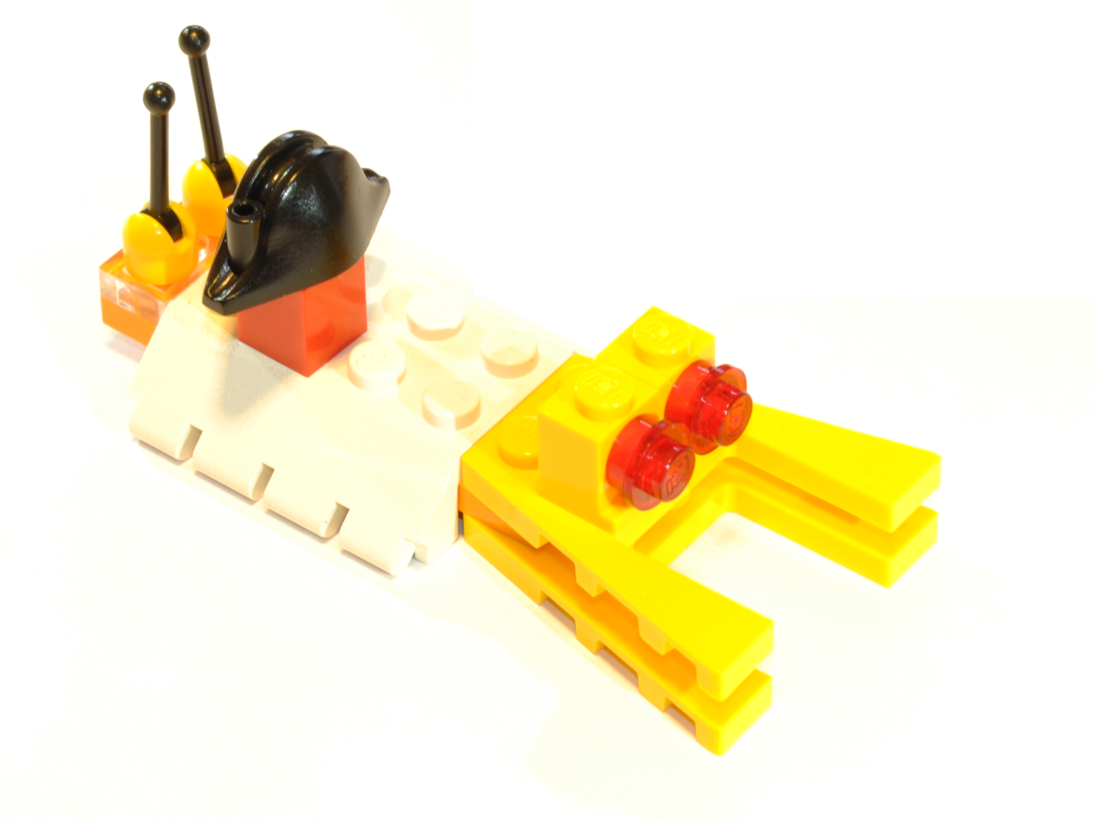
\includegraphics[width=90mm]{images/rawImages/BILD_6}
		\caption{todo.}
		\label{todo}
	\end{figure}
	
	\begin{figure}[ht!]
		\centering
		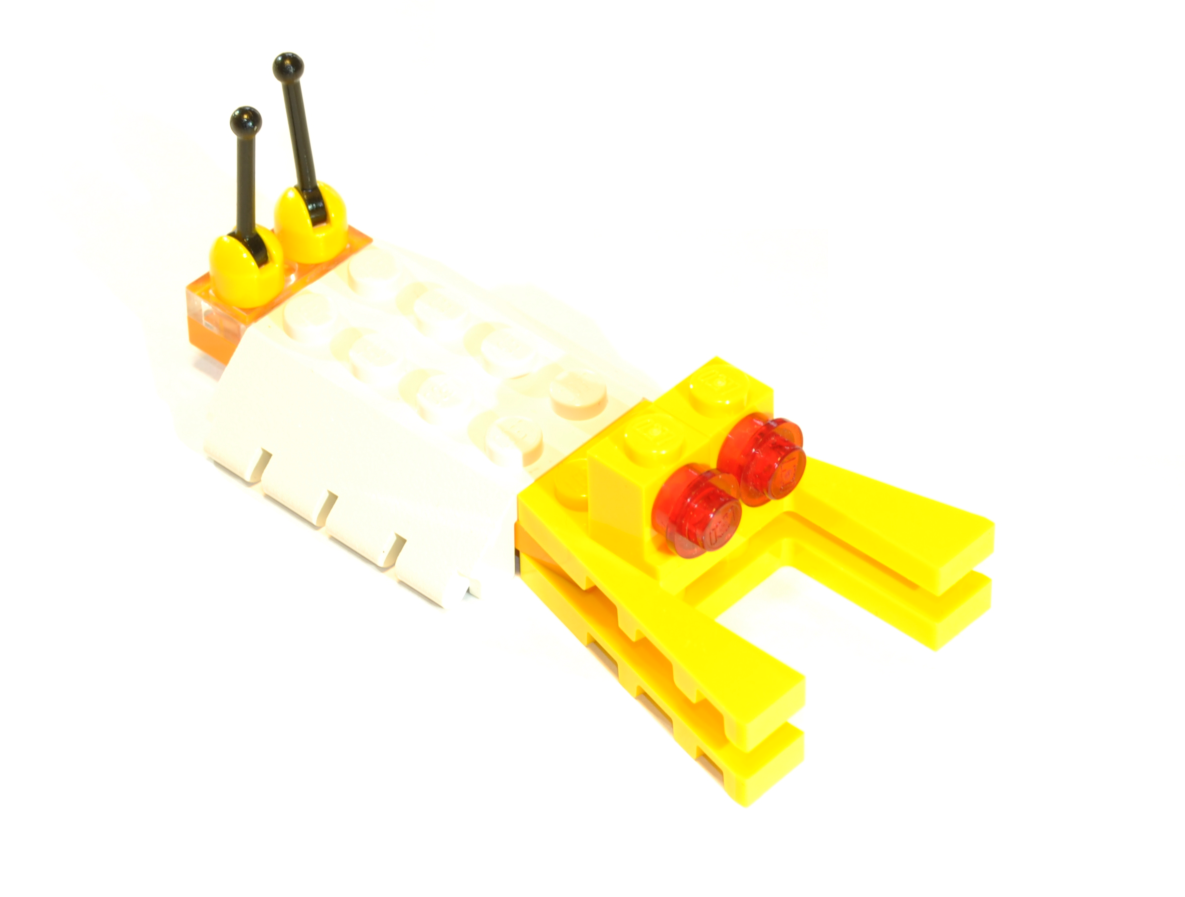
\includegraphics[width=90mm]{images/rawImages/BILD_7}
		\caption{todo.}
		\label{todo}
	\end{figure}
	
	\begin{figure}[ht!]
		\centering
		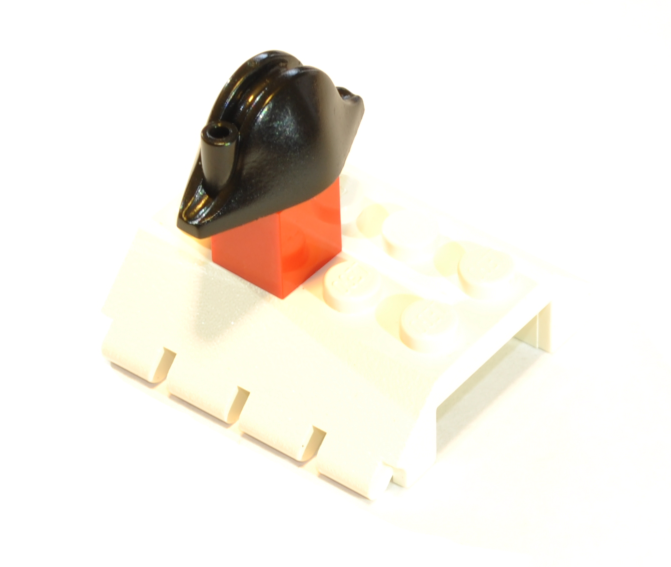
\includegraphics[width=90mm]{images/rawImages/BILD_8}
		\caption{todo.}
		\label{todo}
	\end{figure}